\chapter{Underground Infrastructure}
\label{ch:fscf-und-infra}

The requirements for underground infrastructure for the LBNF Project will be satisfied by a combination of existing infrastructure, improvements to those systems, and development of new infrastructure to suit specific needs. The Project must consider the other tenants underground at SURF for which infrastructure is required, including both the existing Davis Campus experiments and the Ross Campus Experiments. The Ross campus experiments in particular are in relatively close proximity ($\sim$150~m) to LBNF.

The systems must support the LBNF Conventional Facilities (CF) construction activities, Cryogenics Infrastructure, DUNE experiment installation, and operations of both CF Equipment and the experiment. These three scenarios were analyzed and the most demanding requirements chosen from each situation were used to define the requirements for design.

Some of the SURF infrastructure that requires upgrading for LBNF will be rehabilitated prior to the beginning of LBNF construction funding. This includes Ross Shaft rehabilitation, Yates Shaft focused maintenance and repair, and ground support activities at the 4850L between the Yates and Ross Shafts. Additional discussion of this work is included in section 3.5 .

The conceptual underground infrastructure design for LBNF has been performed by several entities. The primary designer referenced in this document is Arup, USA. Arup's scope includes utility provisions and fire protection- life safety (FLS) strategy, covering infrastructure from the surface through the shafts and drifts, to the cavity excavations for the experiment. Utility infrastructure includes fire/life safety systems, permanent ventilation guidance, HVAC, power, plumbing systems, communications infrastructure, lighting and controls, per the experimental utility requirements provided by DUNE and through coordination with LBNF, SURF and the excavation and surface design teams. The design is described in Arup's LBNF 100\% Preliminary Design Report\cite{arup:fscf100pdr} and in the conceptual design drawings. This chapter summarizes the work done by Arup and utilizes information from that report.

Shaft rehabilitation and waste rock handling design were previously provided for the DUSEL PDR. This chapter uses excerpts from the DUSEL Preliminary Design Report, Chapter 5.4 [10]. The research supporting this work took place in whole or in part at the Sanford Underground Laboratory at Homestake in Lead, South Dakota. Funding for this work was provided by the National Science Foundation through Cooperative Agreements PHY-0717003 and PHY-0940801. The assistance of the Sanford Underground Laboratory at Homestake and its personnel in providing physical access and general logistical and technical support is acknowledged.

%%%%%%%%%%%%%%%%%%%%%%%%%%%%%%%%%%%%%%%%%%%%%%%%%%%%%%%%%%%%%%%%%%%
\section{Fire/Life Safety Systems }
\label{sec:fscf-und-fire}

Life safety is a significant design criterion for underground facilities, focusing on events that could impact the ability to safely escape, or if escape is not immediately possible, isolate people from events underground. Design for fire events includes both preventing spread of fire and removing smoke and/or cryogenic gasses through the ventilation system. The evaluation and establishment of requirements for cryogenic gas removal is performed by the cryogenics group and provided to CF.

Life safety requirements were identified and the design developed by Arup, utilizing applicable codes and standards, including NFPA 520: Standard on Subterranean Spaces, which requires adequate egress in the event of an emergency. Facility fire detection and suppression systems, as well as personnel occupancy requirements are defined in accordance with NFPA 101: Life Safety Code. The design was reviewed by Aon Risk Solutions and the recommendations documented in Fire Protection/Life Safety Assessment for the Conceptual Design of the Far Site of the Long Baseline Neutrino Experiment [16]. Due to the unique nature of the experiment and its location, a number of potential variances will require approval from the authority having jurisdiction (AHJ). Significant examples include use of elevators for egress and use of drifts as air \textit{ducts}. The AHJ for Lead, SD is familiar with the facility and the project, and is expected to provide reasonable and timely feedback for proposed variances.  

Based on data provided by SURF the maximum occupant load of the 4850L will be controlled 144 occupants following completion of the Ross Shaft Rehabilitation. This can support the anticipated 42 Underground Operations staff, 50 science staff for LBNF (during installation), and 20 science staff associated with the existing experiments. A logistics study\cite{lbnf-logistics} was completed by Arup evaluating the occupancy load during CF construction as well, confirming the adequacy of this number.

Compartmentation will be needed for egress routes to separate them from adjacent spaces to limit the horizontal and vertical spread of fire and smoke. Use of compartmentation will help to reduce the likelihood of fire and smoke spreading from the area of fire origin to other areas or compartments. Compartmentation will also help limit the spread of other materials such as cryogenic gases, leaks and spills. This results in design criteria of minimum 4-hour fire separation between the LBNF cavities and adjacent drifts, while all rooms that connect directly to the egress drift at 4850L, as well as the shafts, will have 2-hour minimum fire separation.

%%%%%%%%%%%%%%%%%%%%%%%%%%%%%%%%%%%%%%%%%%%%%%%%%%%%%%%%%%%%%%%%%%%
\section{Shafts and Hoists}
\label{sec:fscf-und-shafts}

The Ross and Yates Shafts provide the only access from the surface to the underground, and are therefore critical to the function of the Facility. Both shafts provide service from the surface to the 4850L, though not every intermediate level is serviced from both shafts. The shafts also provide a path for all utilities from the surface to the underground. 

The Ross and Yates Shafts were both installed in the 1930s and have operated since installation. These shafts, along with their furnishings, hoists, and cages, were well maintained during mining operations, but have experienced some deterioration as described in this section. A complete assessment of the Ross and Yates shafts was conducted for the DUSEL Project, and is documented in the Arup Preliminary Infrastructure Assessment Report (DUSEL PDR Appendix 5.M [10]).



%%%%%%%%%%%%%%%%%%%%%%%%%%%%%%%%%
\subsection{Ross Shaft}
\label{sec:fscf-und-shafts-ross}

The Ross Shaft will be used for facility construction, including waste rock removal, routine facility maintenance, and egress path for the finished underground campuses. It will also be used for LBNF experiment primary access. Excavation for LBNF cannot begin until the Ross Shaft is rehabilitated by  SURF.

The Ross Shaft is rectangular in shape --- 14 ft 0 in (4.27 m) by 19 ft 3 in (5.87 m), measured to the outside of the set steel. The shaft collar is at elevation 5,354.88 ft (1,632.17 m) and the 5000L is the bottom level at elevation 277.70 ft (84.64 m) above sea level. Service is provided to 29 levels and five skip loading pockets. The shaft is divided into seven compartments: cage, counterweight, north skip, south skip, pipe, utility, and ladder way. See Figure~\ref{fig:ross-shaft-set} below showing shaft layout.


\begin{cdrfigure}[Ross Shaft, typical shaft set]{ross-shaft-set}{Ross Shaft, typical shaft set (SRK, Courtesy SURF)}
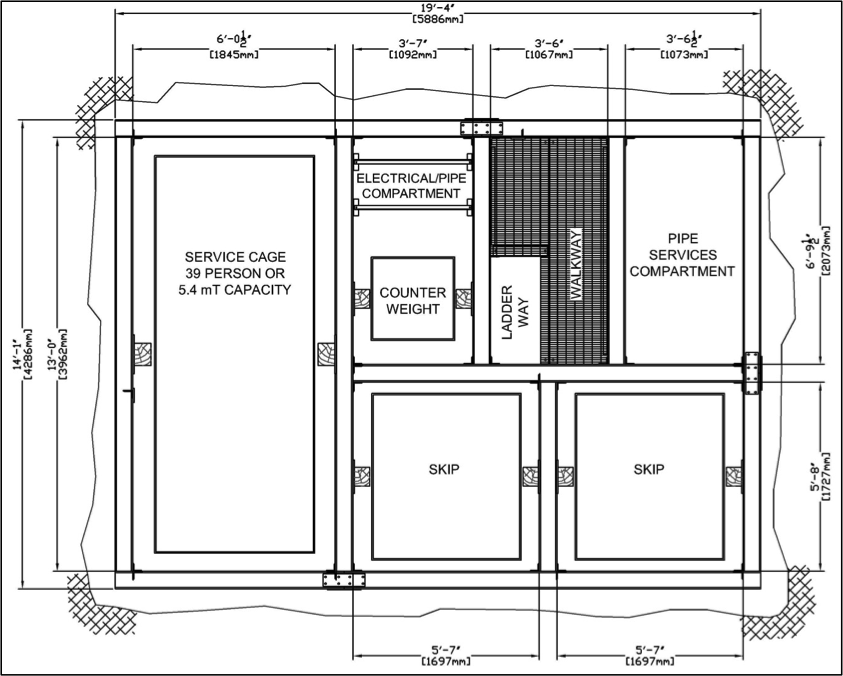
\includegraphics[width=0.8\textwidth]{ross-shaft-set}
\end{cdrfigure}

The Ross Shaft was in operation until the Homestake Gold Mine closed in 2003. Deterioration through corrosion and wear on the shaft steel, including studdles (vertical steel members placed between steel sets), sets, and bearing beams, prompted a full \textit{strip and re-equip} project being performed by  SURF. The Ross Shaft layout will not be significantly modified from the existing configuration. The set spacing is being increased from 6 ft to 18 ft, but the general configuration is remaining the same to allow for emergency egress during rehabilitation. The shaft was installed with limited ground support, electing to utilize lacing to prevent spalled rock from reaching the personnel conveyances. The new design replaces this system with a pattern bolting system to control rock movement. The requirements for this shaft are safety, performance, and code driven and defined by the existing configuration. Shaft rehabilitation through calendar year 2016 has been executed by SURF with non-LBNF Project funds. The rehabilitation is just over 60\% complete as of this report and is planned to be completed in 2017. Beginning in January 2017, the funding for the balance of the rehabilitation project will come from the LBNF project.  This will also include rehabilitation of the skip loading pocket for waste rock handling, and replacement of skips, cage, and ropes..

The production and service hoists at the Ross Shaft are located on the surface in a dedicated hoistroom west of the shaft. The service hoist operates the service cage and the production hoist operates the production skips. The DUSEL PDR describes the condition assessment of the electrical and mechanical hoisting systems which are described in detail in the Arup Preliminary Infrastructure Assessment Report (DUSEL PDR Appendix 5.M [10]). These electrical and mechanical systems will have standard maintenance performed on them to make them in like new condition, but will not be modified from the existing design. The Ross Headframe steel requires some strengthening and modifications to meet code requirements. All of this work is captured in the LBNF scope.

%%%%%%%%%%%%%%%%%%%%%%%%%%%%%%%%%
\subsection{Yates Shaft}
\label{sec:fscf-und-shafts-yates}

The Yates Shaft is rectangular in shape—15 ft-0 in (4.572 m) by 27 ft-8 in (8.433 m) measured to the outside of the set timbers. There are two cage compartments and two skip compartments as shown in Figure~\ref{fig:yates-shaft}. In addition to the cage and skip compartments, there are two other compartments in which shaft services are located. The shaft collar is at 5,310.00 ft (1,618.49 m) elevation and the 4850L is the bottom level at elevation 376.46 ft (114.75 m) above sea level. Service is provided to 18 levels plus four skip-loading pockets. Sets are made up of various length and size timbers located to maintain compartment spaces. The Yates Shaft is timbered except for a fully concrete-lined portion from the collar to the 300L. Recent repairs include full set replacement from the concrete portion to the 800L and additional set repair below this level where deemed critical.

The Yates Service Hoist and Production Hoist are planned to be used as existing, with maintenance performed to bring them into like new condition. Further details regarding the condition of the Yates Hoists' electrical and mechanical condition can be found in Section 2.2 of the Arup Preliminary Site Assessment Report (DUSEL PDR Appendix 5.M) [10].

\begin{cdrfigure}[Existing Yates Shaft layout ]{yates-shaft}{Existing Yates Shaft layout (Adapted from SRK, Courtesy SURF)}
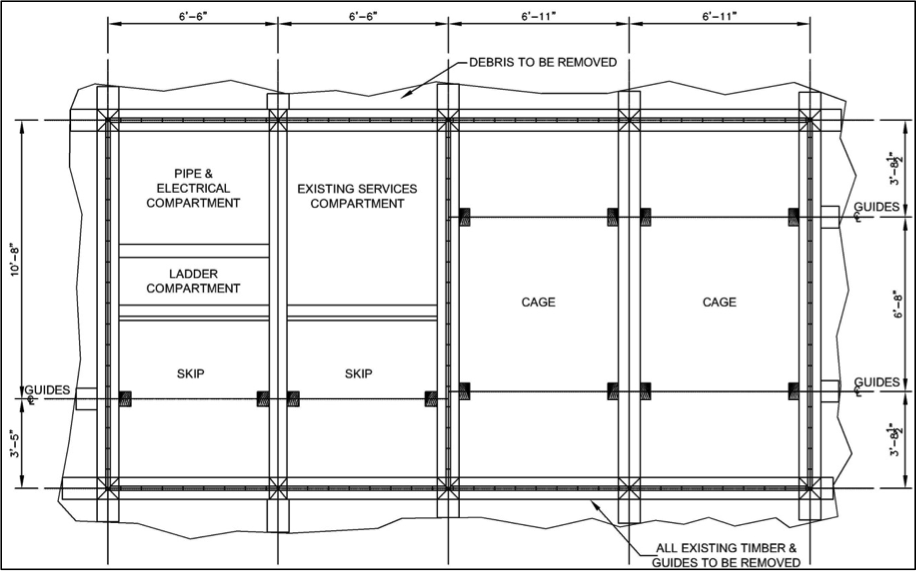
\includegraphics[width=0.8\textwidth]{yates-shaft}
\end{cdrfigure}



%%%%%%%%%%%%%%%%%%%%%%%%%%%%%%%%%%%%%%%%%%%%%%%%%%%%%%%%%%%%%%%%%%%
\section{Ventilation}
\label{sec:fscf-und-vent}

The ventilation system will utilize the existing mine ventilation system for most of the distance to the surface, with modifications made near the LBNF caverns to improve capacity. Fresh air for the LBNF cavities and the utility drifts will be provided by pulling air directly from the existing drifts, which is supplied from the Yates and Ross Shafts. Air will be exhausted from the LBNF cavities and utility drifts through a spray chamber rejecting heat from the LBNF chilled water system into new borehole connecting to the 3500 level of the facility, a short distance from the Oro Hondo shaft, which provide direct connection to the fan at the surface. 230,000 cfm design is required for heat extraction. 27,500 cfm passes through the each main experimental areaand 21,500 through the central utility cavern, with the balance of the air required for heat rejection coming directly from the shafts through connections to existing drifts. The environmental design criteria for LBNF underground spaces are shown in Table~\ref{tab:env-design-crit}.~\footnote{During operations, occupancy of the LBNF cavities is 10. 
Temperature, humidity and filtration requirements in localized areas of these spaces may differ, dependent on requirements. This will be provided by the experiment installation design team. The internal conditions stated above will be used to inform the design of plant and services for each space unless specific requirements that differ from this are provided by LBNF/SURF or the lab experiment design teams.}

\begin{cdrtable}[Environmental design criteria (Arup)]{lllccl}{env-design-crit}{Environmental design criteria (Arup)}
Room & Internal         & Humidity & Min. Vent. Rate/   & Occupancy   \\
         & Temperature & Range     & Fresh Air Changes  & (during assembly)  \\  \toprowrule 

LBNF Cavities & $40 - 82\,^{\circ}\mathrm{F}$ & $15 - 85\%$ & 1& 20(50) \\ 
                      & ($10 - 28\,^{\circ}\mathrm{C}$) & & & \\ \colhline
Access Drifts & Min $50\,^{\circ}\mathrm{F}$ & Uncontrolled & & Transient\\ 
                     & ($10\,^{\circ}\mathrm{C}$) &  & & space \\ \colhline
Utility spaces / & $50 - 95\,^{\circ}\mathrm{F}$ & Uncontrolled & 1& \\ 
Electrical rooms & ($10 - 35\,^{\circ}\mathrm{C}$) &  & & \\ \colhline
Storage Rooms & $59 - 104\,^{\circ}\mathrm{F}$ & Uncontrolled&Min 15 & Room-\\
                        & ($15 - 40\,^{\circ}\mathrm{C}$) & & cfm/person & dependent\\ 
\end{cdrtable}


Per historical data, outdoor temperatures can drop below $-20\,^{\circ}\mathrm{F}$; therefore, the intake air requires heating to prevent ice build-up in the shafts which could potentially disrupt hoisting operations and damage shaft support members, cables and piping. The existing shaft heaters are expected to be adequate for normal operation, but temporary supplemental heating may be necessary during excavation due to higher demands.  A study will be performed during final design to determine if waste heat from the cryogenic systems surface compressors can be used for energy savings to heat the intake air.

%%%%%%%%%%%%%%%%%%%%%%%%%%%%%%%%%%%%%%%%%%%%%%%%%%%%%%%%%%%%%%%%%%%
\section{Electrical}
\label{sec:fscf-und-elec}

The underground facilities at the 4850L will have electrical power for normal operations as well as standby power for emergency occupant evacuation. LAr experiment power requires standby power for circulation of cryogens to avoid rapid boil-off and loss of argon.

%%%%%%%%%%%%%%%%%%%%%%%%%%%%%%%%%%
\subsection{Normal Power}
\label{sec:fscf-und-norm-pwr}

The estimated electrical loads for both the far detector experiment and the underground infrastructure serving the experimental spaces are included in the facility load determination and design. 

Power to serve the far detector experiment will originate from the Ross substation and be routed down the Ross Shaft to the 4850L. One set of 15-kV mining cables shall be installed down the Ross Shaft to the 4850L and shall be cable rated for mine use, highly flame retardant, low smoke toxicity with high tensile strength and self-supporting. At the 4850L, the 15-kV mining cables will terminate in 15-kV switchgear located in a new Ross underground substation. This will be provided early in the construction process to allow it to be used for construction.

%%%%%%%%%%%%%%%%%%%%%%%%%%%%%%%%%%
\subsection{Standby and Emergency Power}
\label{sec:fscf-und-emerg-pwr}

A 300kW emergency/standby diesel generator will be provided in the Central Utility Cavern to serve standby and emergency loads. 48 hours of diesel fuel will be provided to operate the generator when surface power is inoperable. This duration aligns with the stored LN for controlling argon boil off, both of which were derived from historical power outages at the facility.  Note that the facility is fed by the local utility provider in a loop infrastructure, and therefore power to the site has historically been very reliable -- on the order of a few hours down per year.  Within the facility, power outages due to maintenance or unforeseen events are also at a very low rate.  The following 4850L electrical loads are anticipated to be installed to the emergency/standby power system:

\begin{itemize}
\item Security
\item IT System for communications
\item Smoke control fans
\item Mono rail
\item Cryostat system controls
\end{itemize}

%%%%%%%%%%%%%%%%%%%%%%%%%%%%%%%%%%
\subsection{Fire Alarm and Detection}
\label{sec:fscf-und-fire-alarm}

The 4850L will have notification devices installed to alarm the occupants of a fire. Notification devices will consist of speakers and strobe lights. Manual pull stations will be provided within 200 ft of egress. Phones will be installed in the liquid argon chambers and every 400 ft along the access drifts to communicate with the surface level command center.

An air sampling and gas detection system will be installed in the drifts and liquid argon detector chamber as an early detection of a fire condition. The air sampling system will be connected into the fire alarm system.

The fire alarm system will also interface with the oxygen deficiency hazard (ODH) system to activate the fire alarm system and initiate an alarm at the respective level fire alarm panel and at the surface level command center. Specific sounds and strobe colors will be identified based on the type of alarm (fire, ODH, etc.).

%%%%%%%%%%%%%%%%%%%%%%%%%%%%%%%%%%
\subsection{Lighting}
\label{sec:fscf-und-light}

Suspended lights mounted at a height just below the lowest obstruction will be provided for all drifts and ramps. Mounting is to be coordinated with conduit and supports of other systems running overhead. Maintained average illumination of approximately 24 lux (2.4 foot candles) at floor level will be provided throughout the drifts. Lighting control in drifts will be via low voltage occupancy sensors and power packs suitable for high humidity environments.

%%%%%%%%%%%%%%%%%%%%%%%%%%%%%%%%%%
\subsection{Grounding}
\label{sec:fscf-und-grounding}

The grounding system will be designed to provide effective grounding to enable protective devices to operate within a specified time during fault conditions, and to limit touch voltage under such conditions. The grounding system will be designed for a maximum resistance of 5 ohms where possible based on Mine Safety and Health Administration (MSHA) recommendations for ground resistance in mines. Ground beds, consisting of an array of ground rods, will be installed at each substation to provide low impedance to ground.

Electrical separation between the cryostat detectors and cavern utilities will be achieved by separating the metal components (rebar, structure support, etc.) from each other. Inductors will be installed between grounding systems to control noise between systems while also controlling touch potential for safety.

%%%%%%%%%%%%%%%%%%%%%%%%%%%%%%%%%%%%%%%%%%%%%%%%%%%%%%%%%%%%%%%%%%%
\section{Plumbing}
\label{sec:fscf-und-plumbing}

Plumbing provided by CF, but specific to DUNE, includes plumbing for the cooling systems and gas piping for nitrogen and argon delivery from the Cryogenics Compressor Building on surface to the Central Utility Cavern. Beyond this the facility requires supplies of both potable and industrial water, as well as a means to remove water inflows. 

%%%%%%%%%%%%%%%%%%%%%%%%%%%%%%%%%%
\subsection{Industrial Water}
\label{sec:fscf-und-ind-h2o}

An existing 4-inch industrial water riser will be used for construction and as a secondary fire service. It is not feasible to run an uninterrupted main water supply line from grade level down to serve the lower levels due to the extremely high hydrostatic pressure that would occur in the system. A series of pressure reducing stations are located at regular intervals in intermediate levels and at the 4850L in order to maintain the pressure within the capability of readily available piping.

%%%%%%%%%%%%%%%%%%%%%%%%%%%%%%%%%%
\subsection{Potable Water}
\label{sec:fscf-und-pot-h2o}

Potable water is not required in large quantities for LBNF. The SURF experience has been that plumbing potable water through the shafts for low volumes is not effective, as the pressure reducing systems have the potential to introduce biological contaminants that result in the water no longer meeting drinking water standards, especially in low flow situations. To address this, local filters and ultraviolet treatment is done at the 4850L to make industrial water meet drinking water standards. This system has been used successfully for several years at SURF.

%%%%%%%%%%%%%%%%%%%%%%%%%%%%%%%%%%
\subsection{Chilled Water}
\label{sec:fscf-und-ch-h2o}

The DUNE equipment will produce a significant amount of heat which will be removed by LBNF-provided chillers. Three chillers at 50\% each have been selected to provide N+1 redundancy to allow for maintenance. Heat from the chillers and various process loads will be rejected using a spray chamber located at the east end of the 4850L LBNF caverns immediately before exhausting into a new borehole providing a direct connection to the exhaust shaft to surface. The ventilation air is a mixture of air from the Yates and Ross Shafts at approximately 68 degrees F. This volume of air is such that the total heat rejected (2.9 MW or 822 Ton) will raise the air temperature to no more than 95 degrees F. 

%%%%%%%%%%%%%%%%%%%%%%%%%%%%%%%%%%
\subsection{Fire Suppression}
\label{sec:fscf-und-fire-supp}

The source of fire water main will be the existing 4-inch industrial water main at Ross Shaft. The connection to this line will be at the 4100L, where a new sump with at least 27,000 gallons capacity will be built using sump walls in an existing drift to provide 90 minutes of capacity even if the supply were cut off. The fire protection system at the 4850L Campus will be a gravity fed system. There will be a connection to an existing 6-in industrial water main in the west drift fed from Yates Shaft, where a similar, but slightly larger at 50,000 gallons, sump has been built by SURF. This provides redundant supply from surface.

%%%%%%%%%%%%%%%%%%%%%%%%%%%%%%%%%%
\subsection{Drainage}
\label{sec:fscf-und-drain}

Drainage [17] from the drifts, mechanical electrical rooms (MERs), and any areas where spillage is likely to occur will be collected locally in sumps. Sumps will be located every 500 feet in any areas where drainage to the drifts is not practical. Sumps will be equipped with sump pumps in a staged configuration where each pump discharging to the adjacent sump until water is discharged to the \#6 Winze, where it flows to the primary facility pool approximately 1,000 feet below the 4850L. From there, the existing SURF dewatering system pumps the water in stages to the surface where it is treated before discharge into a nearby stream.

%%%%%%%%%%%%%%%%%%%%%%%%%%%%%%%%%%
\subsection{Sanitary Drainage}
\label{sec:fscf-und-san-drain}

No sanitary drainage is included in the requirements for LBNF. Existing SURF facilities are planned to be used.

%%%%%%%%%%%%%%%%%%%%%%%%%%%%%%%%%%
\subsection{Nitrogen and Argon Gas Piping}
\label{sec:fscf-und-gas-piping}

Two 16-in and three 8-in mild steel pipes are provided by CF from the surface Cryogenics Compressor Building to the shaft, through the shaft, and across the 4850L to the Central Utility Cavern west entrance. The design and specifications of this piping are the responsibility of the Cryogenics Infrastructure Project team. The supply and installation within the Cryogenics Compressor Building and the central Utility Cavern is also the responsibility of the Cryogenics Infrastructure Project.


%%%%%%%%%%%%%%%%%%%%%%%%%%%%%%%%%%%%%%%%%%%%%%%%%%%%%%%%%%%%%%%%%%%
\section{Cyberinfrastructure}
\label{sec:fscf-und-cyber}

The Structured Cable System design will be based on uniform cable distribution with a star topology. New fiber connections will be extended to the 4850 level from the Ross Dry Building, and will be dedicated to the use of LBNF experiments at the 4850 level.The design provides one (1) 96-strand single mode armored fiber optic cable from the DUNE Control room dedicated to the experiments. A second 96 stand single mode armored fiber optic cable will be routed through the Yates shaft to provide redundancy for data systems.  Figure~\ref{fig:fiber-distrib} shows the fiber distribution network for LBNF.

\begin{cdrfigure}[Fiber distribution system for LBNF]{fiber-distrib}{Fiber distribution system for LBNF (Arup)}
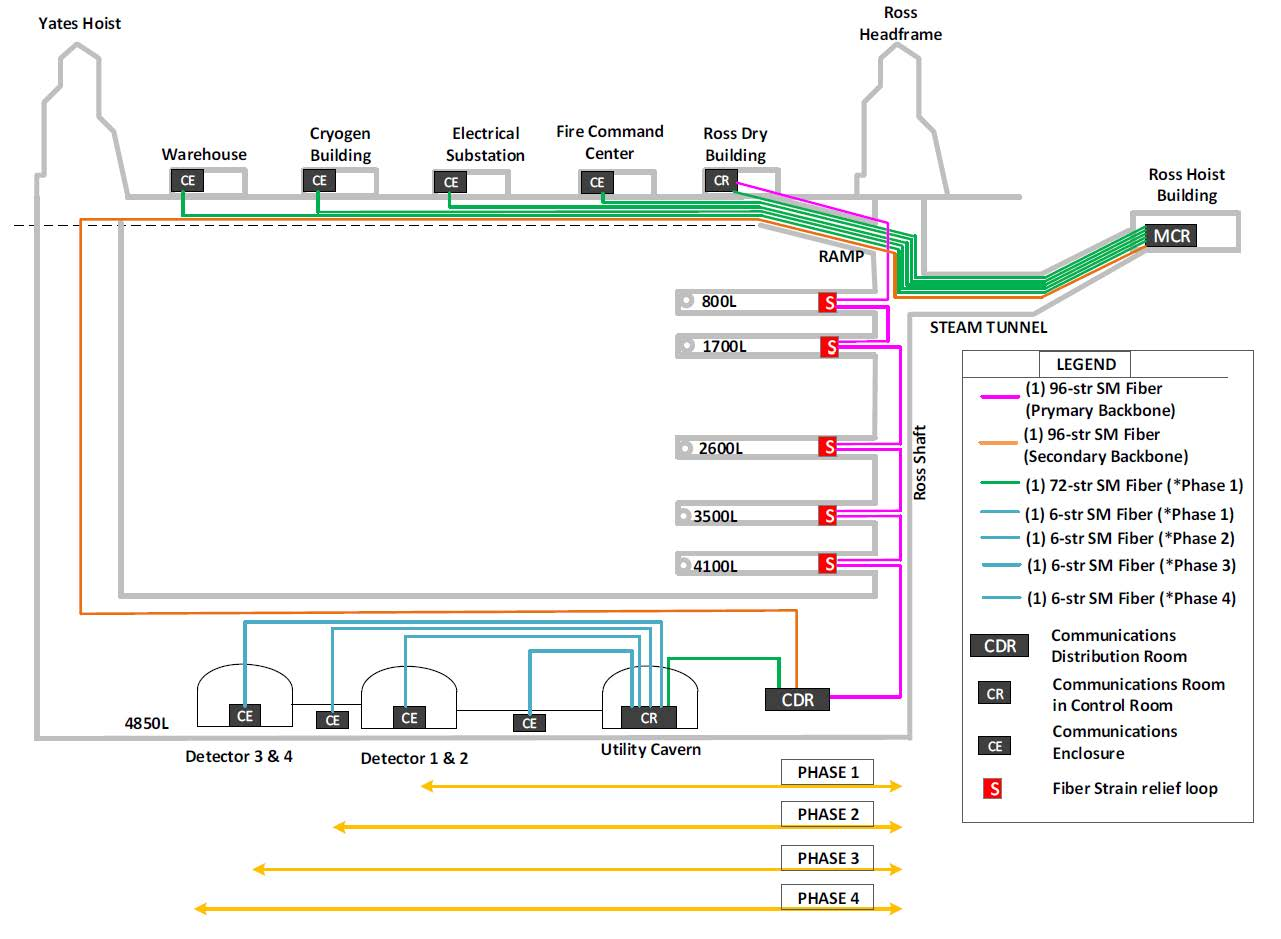
\includegraphics[width=0.8\textwidth]{fiber-distrib}
\end{cdrfigure}

Voice communications are provided via two-way radios and phones distributed throughout the underground spaces (in every room as well as every 500 ft in drifts). Two-way radios and cellular phones utilize a leaky feeder system to ensure communications over long distance without line of site. These leaky feeders are cables that act as antennas installed the length of all drifts and shafts. Standard phones utilize Voice over Internet Protocol (VoIP) to provide communication though the fiber optic data backbone.

The data system is designed to provide 10-Gigabit Ethernet in the backbone and 1-Gigabit Ethernet to connected systems (computers). This system is intentionally left at a lesser level of design due to the continuous progression and advancement of technology that will almost certainly result in more advanced technologies than are currently available being utilized at the time of construction.

%%%%%%%%%%%%%%%%%%%%%%%%%%%%%%%%%%%%%%%%%%%%%%%%%%%%%%%%%%%%%%%%%%%
\section{Waste Rock Handling }
\label{sec:fscf-und-waste-rock}

Prior to the commencement of any excavation activities, it will be necessary to establish a waste rock handling system \fixme{Josh says: Need to determine whether this terminology is acceptable from Pepin}. The capacity of this system will be equivalent to what was in place during mining. 
There are a number of components to the waste rock handling system, including refurbishing the Ross Shaft hoisting system, the Ross Shaft crushers, and a new conveying system to transport rock downhill to the Kirk Road, as seen in Figure~\ref{fig:waste-rock-sys}. 

\begin{cdrfigure}[Waste rock handling system route]{waste-rock-sys}{Waste rock handling system route (SRK, Courtesy SURF)}
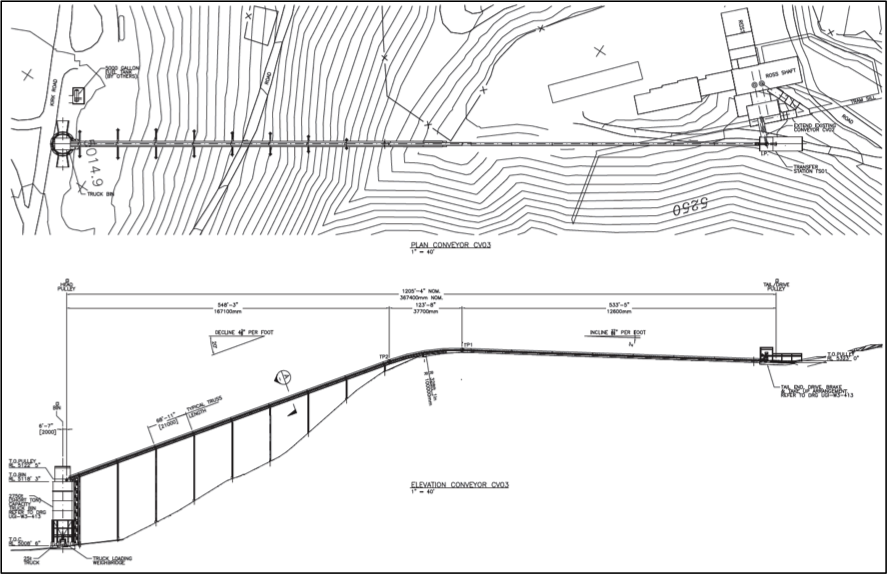
\includegraphics[width=0.8\textwidth]{waste-rock-sys}
\end{cdrfigure}

The systems utilize experience and equipment from the former Homestake Mining Company legacy, where rock was removed to the surface using skips in both the Yates and Ross Shafts. At the headframe of each shaft, the material was crushed to a nominal $3/4$~in, passed through ore bins, and was transported via underground rail to the mill system. All systems from the underground to the crushers will be rehabilitated from the original systems, though the material may not be required to be crushed as fine as it was historically, and therefore some components of the system may not be re-used.



